\documentclass[11pt,a4paper]{article}
\usepackage[margin=24mm,headheight=14pt]{geometry}
\usepackage{amsmath,amssymb,graphicx,booktabs,tabularx,array,float}
\usepackage{caption,fancyhdr,eso-pic,needspace,listings,xcolor}
\usepackage[hidelinks,breaklinks]{hyperref}
\usepackage[T1]{fontenc}
\usepackage{lmodern}
\usepackage{microtype}
\setlength{\parindent}{1.3em}
\setlength{\parskip}{4pt}
\setlength{\emergencystretch}{2em}
\linespread{1.08}
\setcounter{secnumdepth}{2}
\captionsetup{font=small,labelfont=bf,justification=centering}
\pagestyle{fancy}
\fancyhf{}
\fancyhead[L]{\small EN4594 -- Autonomous Systems}
\fancyhead[R]{}
\fancyfoot[C]{\thepage}
\renewcommand{\headrulewidth}{0.3pt}
\lstset{basicstyle=\ttfamily\footnotesize,breaklines=true,columns=fullflexible,keepspaces=true,frame=single,framerule=0.3pt,showstringspaces=false,aboveskip=8pt,belowskip=8pt}
\newcolumntype{Y}{>{\raggedright\arraybackslash}X}
\AddToShipoutPictureBG{\AtPageLowerLeft{\put(28.35,28.35){\setlength{\unitlength}{1pt}\linethickness{0.4pt}\framebox(538.57,785.19){}}}}
\begin{document}
\begin{titlepage}
\hypersetup{pageanchor=false}
\centering
\vspace*{6mm}

\includegraphics[height=43mm]{assets/uom_emblem.jpg}\par
\vspace{7mm}
{\Large University of Moratuwa\par}
\vspace{3mm}
{\Large Faculty of Engineering\par}
\vspace{3mm}
{\large Department of Electronic and Telecommunication Engineering\par}
\vspace{13mm}
{\large EN4594\par}
\vspace{2mm}
{\large Autonomous Systems\par}
\vspace{11mm}
{\huge\bfseries Mini Project Report\par}
\vspace{8mm}
{\LARGE\bfseries Kalmann Filter Based Distance and Relative Speed Estimation for Autonomous Vehicle Safety\par}
\vspace{14mm}
{\Large Manawadu M.D\par}
\vspace{3mm}
{\large Index Number: 220381M\par}
\vspace{4mm}
{\large 27 October 2026\par}
\vfill
{\large\bfseries Source Code Repository\par}
\vspace{3mm}
{\small\url{https://github.com/Demitha-Manawadu/Autonomous-Mini-Project.git}\par}
\vspace{10mm}
\end{titlepage}
\hypersetup{pageanchor=true}
\pagenumbering{roman}
\setcounter{tocdepth}{2}
\renewcommand{\contentsname}{Table of Contents}
\tableofcontents
\clearpage
\pagenumbering{arabic}

\clearpage\section{Introduction}
\needspace{4\baselineskip}\subsection{Project background}
A vehicle needs to know how far an object is ahead and how quickly that gap is closing. These quantities support following-distance warnings and braking decisions. A noisy sensor can make the distance fluctuate. Estimating relative speed by subtracting consecutive readings makes the noise worse.\par

We selected a linear Kalman filter to estimate distance and relative speed from range measurements. We tested it in two road scenarios: following a moving vehicle that brakes and approaching a stationary obstacle. A simple braking controller uses the estimated states to respond to closing traffic.\par

\needspace{4\baselineskip}\subsection{Why this application was selected}
The application connects state estimation to a clear vehicle-safety problem. Both estimated quantities have a direct meaning: the gap tells how much space remains, and relative speed tells whether that space is shrinking. Moving and stationary targets also provide two different tests of the same estimator. Simulation makes it possible to compare each estimate with the exact state without requiring a vehicle or range-sensor hardware.\par

\needspace{4\baselineskip}\subsection{Why a linear Kalman filter was selected}
For motion along one lane, the distance and relative-speed equations are linear. The range sensor measures distance directly, so the measurement model is linear too. A standard KF therefore fits the chosen model. An Extended KF would add linearisation without a need for it here. A Particle Filter would require a population of samples for a problem that can be represented by two state values and a covariance matrix.\par

The KF combines a motion prediction with each new sensor reading. It can estimate relative speed even though the sensor measures only distance. It also reports uncertainty and can predict through short gaps in the observations. Its small computational cost makes it suitable for repeated updates.\par

\needspace{4\baselineskip}\subsection{Objectives and scope}
The work aims to derive and implement the filter, demonstrate both road scenarios, measure errors against simulated truth, and examine tuning and sensor loss. The main question is whether filtering improves distance and relative-speed estimates compared with simple raw baselines.\par

The model is longitudinal and tracks one known in-lane object. It does not perform mapping or steering. Lane membership is supplied by the simulator. Python is used for motion, measurements, filtering and plotting; the KF itself is implemented directly with matrix operations.\par

\clearpage\section{Methodology}
\needspace{4\baselineskip}\subsection{Simulation arrangement}
\needspace{4\baselineskip}\subsubsection{Sensor, filter and controller}
\begin{lstlisting}
Vehicle motion -> noisy range sensor -> KF estimate
                                      -> risk check -> ego braking
Ground truth --------------------------> error evaluation only
\end{lstlisting}
The simulated sensor measures the bumper-to-bumper gap to a known object in the lane. It has a forward range of 180 m. Zero-mean Gaussian noise is added to each valid reading. The default standard deviation is 2 m. The KF receives these readings, not the true target position or speed.\par

\needspace{4\baselineskip}\subsubsection{What the road display means}
The ego rectangle is blue and turns red during braking. The target is green. A cyan line represents the sensor beam. Red crosses show measured target position; the orange marker shows the KF estimate. Gray blocks are fixed roadside objects. Magenta rings mark visible roadside objects.\par

Roadside ranges are also generated and saved. Object identity and lane membership are supplied by the simulator. Objects outside the lane do not enter the in-lane target filter. This simplifies detection; no camera recognition or multi-object association is implemented.\par

Both vehicles move in a fixed world coordinate system. In the following case, both rectangles advance along the road. In the obstacle case, only ego advances and the target stays fixed. The earlier ego-centred view was also valid, but a fixed road makes movement easier to see.\par

Figure captions identify the scenario, sample time and seed. The numerical results use ground truth only for evaluation; the estimator and braking decision do not use the true target state.\par

\begin{figure}[H]\centering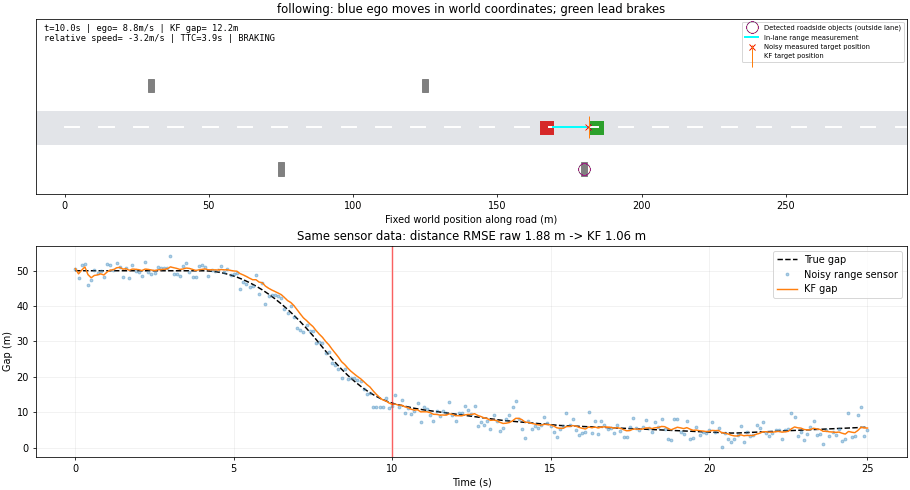
\includegraphics[width=0.957\linewidth]{assets/following_gif_frame.png}\caption{Frame from the exported following-scenario GIF at approximately 10 s. The upper view shows vehicle positions and sensor markers. The lower plot shows the true, measured and filtered gap, with a red cursor marking playback time.}\end{figure}
\clearpage
\needspace{4\baselineskip}\subsection{Important parameters and scenario design}
Table 1 lists the main settings. The values define a manageable demonstration and are not claimed to be validated automotive limits. Both scenarios use the same filter and sensor settings.\par

\begin{table}[H]\centering\caption{Main simulation and filter parameters.}\small\renewcommand{\arraystretch}{1.2}\begin{tabularx}{\linewidth}{YYY}\toprule
\textbf{Parameter} & \textbf{Value} & \textbf{Purpose} \\
\midrule
Duration / sample interval & 25 s / 0.1 s & 251 samples; 10 updates per second \\
Range noise standard deviation & 2 m & Uncertainty in each range observation \\
Process acceleration standard deviation & 2 m/s\textsuperscript{2} & Allows changes not captured by prediction \\
Sensor forward range & 180 m & Limits valid forward observations \\
Initial relative-speed variance & 100 (m/s)\textsuperscript{2} & Represents unknown speed at start-up \\
Initial ego speed & 18 m/s & Same initial speed in both road cases \\
Following initial gap & 50 m & Both vehicles initially travel at 18 m/s \\
Lead braking & -3 m/s\textsuperscript{2} at 4--8 s & Lead reaches 6 m/s \\
Stationary target position & 100 m & Fixed in-lane obstacle; target speed is zero \\
Ego braking command & -4 m/s\textsuperscript{2} & Ideal deceleration; speed limited to zero \\
Braking TTC threshold & 5 s & Applied when closing faster than 0.3 m/s \\
Stationary-target gap rule & Estimated gap < 12 m & Maintains braking near the fixed obstacle \\
Noise seeds & 42--61 & 20 repeated trials per road scenario \\
\bottomrule\end{tabularx}\end{table}
\needspace{4\baselineskip}\subsubsection{Reasons for the settings}
The 0.1 s interval provides a clear sequence of distance observations while keeping the animation easy to follow. The 25 s run includes motion before braking, the braking event and the response afterwards. A 2 m noise standard deviation makes measurement scatter visible, so the effect of filtering can be measured.\par

Process uncertainty is set to 2 m/s\textsuperscript{2} as a starting value and is varied later. It is a tuning parameter rather than a measured acceleration. The initial speed variance is large because one distance reading cannot reveal closing speed. The TTC and brake settings give a simple link between estimated motion and action, while keeping controller complexity outside the main filter study.\par

The following case tests target braking. The stationary case tests a large initial closing speed and the transition to rest.\par

\clearpage
\needspace{4\baselineskip}\subsection{Mathematical model}
\needspace{4\baselineskip}\subsubsection{State and sign convention}
The state contains the gap in metres and relative speed in metres per second. Relative speed is target speed minus ego speed. A negative value means the gap is closing.\par

\begin{equation}\mathbf{x}_k=\begin{bmatrix}d_k\\v_{r,k}\end{bmatrix},\qquad v_{r,k}=v_{t,k}-v_{e,k}\end{equation}
\begin{equation}\begin{aligned}d_{k+1}&=d_k+\Delta t\,v_{r,k}+\tfrac12\Delta t^2 u_k,\\v_{r,k+1}&=v_{r,k}+\Delta t\,u_k.\end{aligned}\end{equation}
These equations follow from one-dimensional motion over a short interval. In the road scenarios, u is minus the known executed ego acceleration. Unknown target acceleration is represented by process uncertainty. The sensor model is linear, so an Extended KF is not required.\par

\needspace{4\baselineskip}\subsubsection{State-space form}
\begin{equation}\mathbf{x}_{k+1}=\mathbf{F}\mathbf{x}_k+\mathbf{G}u_k+\mathbf{w}_k,\qquad z_k=\mathbf{H}\mathbf{x}_k+n_k\end{equation}
\begin{equation}\mathbf{F}=\begin{bmatrix}1&\Delta t\\0&1\end{bmatrix},\quad\mathbf{G}=\begin{bmatrix}\Delta t^2/2\\\Delta t\end{bmatrix},\quad\mathbf{H}=\begin{bmatrix}1&0\end{bmatrix},\quad u_k=-a_{e,k}\end{equation}
With a positive time step, the two rows H and HF form an observability matrix with determinant dt. It therefore has rank two. This explains why relative speed can be estimated from a sequence of distance observations even when the sensor does not measure speed.\par

\needspace{4\baselineskip}\subsubsection{Noise and initial uncertainty}
\begin{equation}\mathbf{Q}=\sigma_a^2\mathbf{G}\mathbf{G}^{\mathsf T},\quad R=\sigma_z^2,\quad \mathbf{w}_k\sim\mathcal{N}(\mathbf{0},\mathbf{Q}),\quad n_k\sim\mathcal{N}(0,R)\end{equation}
\begin{equation}\widehat{\mathbf{x}}_0=\begin{bmatrix}z_0\\0\end{bmatrix},\qquad\mathbf{P}_0=\begin{bmatrix}R&0\\0&100\end{bmatrix}\end{equation}
Using a 0.1 s sample interval, a process acceleration standard deviation of 2 m/s\textsuperscript{2} and a range standard deviation of 2 m gives the following covariances.\par

\begin{equation}\mathbf{Q}=\begin{bmatrix}0.0001&0.002\\0.002&0.04\end{bmatrix},\qquad R=4\ \mathrm{m^2}\end{equation}
The process model assumes an independent random relative acceleration held constant within each sample interval. Its tuning depends on the sampling interval.\par

Initial relative speed is unknown and is set to zero with a large variance of 100 (m/s)\textsuperscript{2}. The first observation initializes distance and is not applied again as a correction. This avoids counting the same measurement twice.\par

\clearpage
\needspace{4\baselineskip}\subsection{Kalman filter and braking decision}
\needspace{4\baselineskip}\subsubsection{Predict}
\begin{equation}\widehat{\mathbf{x}}_k^- =\mathbf{F}\widehat{\mathbf{x}}_{k-1}+\mathbf{G}u_{k-1},\qquad\mathbf{P}_k^-=\mathbf{F}\mathbf{P}_{k-1}\mathbf{F}^{\mathsf T}+\mathbf{Q}\end{equation}
Prediction moves the estimated state forward by one sample. The known ego acceleration accounts for the motion of the observer. Covariance P describes uncertainty in the state. Adding Q allows the estimate to change when the target does not follow the expected motion.\par

\needspace{4\baselineskip}\subsubsection{Correct with the sensor reading}
\begin{equation}y_k=z_k-\mathbf{H}\widehat{\mathbf{x}}_k^-,\qquad S_k=\mathbf{H}\mathbf{P}_k^-\mathbf{H}^{\mathsf T}+R\end{equation}
\begin{equation}\mathbf{K}_k=\mathbf{P}_k^-\mathbf{H}^{\mathsf T}S_k^{-1},\qquad\widehat{\mathbf{x}}_k=\widehat{\mathbf{x}}_k^-+\mathbf{K}_k y_k\end{equation}
The innovation is the difference between the observed and predicted distance. The Kalman gain K sets how much that difference changes distance and relative speed. A larger R gives less weight to a reading. Greater predicted uncertainty generally gives it more weight.\par

\needspace{4\baselineskip}\subsubsection{Update uncertainty}
\begin{equation}\mathbf{P}_k=(\mathbf{I}-\mathbf{K}_k\mathbf{H})\mathbf{P}_k^-(\mathbf{I}-\mathbf{K}_k\mathbf{H})^{\mathsf T}+\mathbf{K}_kR\mathbf{K}_k^{\mathsf T}\end{equation}
This is the Joseph covariance update. It is used to reduce numerical problems with covariance symmetry and non-negative uncertainty. When a reading is missing, the correction is skipped. Only the predicted state and covariance are kept.\par

\needspace{4\baselineskip}\subsubsection{Time to collision and braking}
\begin{equation}\operatorname{TTC}=\begin{cases}0,&d\leq0,\\d/(-v_r),&d>0,\ v_r<-0.1\ \mathrm{m\,s^{-1}},\\\infty,&\text{otherwise}.\end{cases}\end{equation}
For example, a 20 m gap closing at 5 m/s gives a TTC of 4 s. The road controller commands -4 m/s\textsuperscript{2} when estimated TTC is below 5 s and estimated closing speed exceeds 0.3 m/s. In the known stationary-obstacle case, an estimated gap below 12 m also maintains braking. Ego speed cannot become negative.\par

TTC is calculated after the KF update. It assumes relative speed stays unchanged. The controller is a small demonstration of how estimates can be used; it is not a validated emergency-braking system.\par

\clearpage\section{Implementation}
\needspace{4\baselineskip}\subsection{Files and libraries}
\begin{table}[H]\centering\caption{Main implementation components.}\small\renewcommand{\arraystretch}{1.2}\begin{tabularx}{\linewidth}{YY}\toprule
\textbf{Part} & \textbf{Purpose} \\
\midrule
simulation.py / NumPy & KF matrices, prediction, correction, TTC and errors \\
road.py / NumPy & Vehicle motion, noisy sensor and brake response \\
road.py / Matplotlib & Road rectangles and FuncAnimation playback \\
main.py & Commands, plots and CSV/JSON export \\
Pillow & Optional animated GIF export \\
test\_\allowbreak{}simulation.py & Seven automated checks \\
\bottomrule\end{tabularx}\end{table}
\needspace{4\baselineskip}\subsection{Generating a moving object}
\begin{lstlisting}
ego_speed[k+1] = max(0., ego_speed[k] + acceleration[k]*dt)
ego[k+1] = ego[k] + 0.5*(ego_speed[k] + ego_speed[k+1])*dt

gap = lead[k] - ego[k]
measurement[k] = gap + noise[k]
\end{lstlisting}
This excerpt follows the road simulation code, using dt for c.dt. Speed is updated first. Position is then advanced using average speed. At 18 m/s, a vehicle travels about 1.8 m in one 0.1 s step. A stationary obstacle keeps the same position. The ego position marks its front bumper, while target position marks its rear bumper.\par

\needspace{4\baselineskip}\subsection{Connecting the KF and animation}
\begin{lstlisting}
actual_ego_accel = (ego_speed[k] - ego_speed[k-1]) / dt
estimate[k], covariance[k], innovation[k] = (
    kf.step(measurement[k], -actual_ego_accel)
)
# Animation places rectangles at the stored positions:
ego_rectangle.set_x(ego_position - 4.5)
\end{lstlisting}
The acceleration expression applies after the first sample; the initial value is zero. In this ideal simulator executed ego acceleration is available without error. The filter never receives true target speed or true gap.\par

The full trajectory is calculated before animation starts. Each sample still follows a causal sensor-update-control sequence. Matplotlib then plays those stored states at approximately real-time speed. Replaying the animation does not run new sensor samples. A different random seed produces another noise realization.\par

Running this two-state KF is inexpensive. A local timing check averaged about 17 microseconds per update over 10,000 updates, excluding graphics. This is an illustrative timing, not a portable benchmark. The challenging work is modelling, tuning and validation, rather than the small matrix calculation.\par

\clearpage
\needspace{4\baselineskip}\subsection{Run the demonstrations}
\begin{lstlisting}
python -m pip install -r requirements.txt
python main.py --demo

# Individual scenarios
python main.py --scenario following
python main.py --scenario obstacle

# Repeated trials and verification
python main.py --demo --headless --trials 20 --output outputs/road_trials
python -m unittest -v
\end{lstlisting}
The demonstration command calculates fresh trajectories and then opens the comparison plots and repeating animations. Seed 42 is the default. Add --seed 73, for example, to change the measurement noise. Add --headless to save plots without opening windows, or --gif to export animation.\par

results.csv contains truth, measurements, estimated states, uncertainty and TTC. road\_\allowbreak{}sensor.csv contains world positions, vehicle speeds, brake commands and roadside ranges. metrics.json and summary.csv contain numerical results. The report\_\allowbreak{}evidence.json file in the report folder stores the exact repeated-trial and tuning values used for this report.\par

\needspace{4\baselineskip}\subsection{Source code}
\noindent Source code: \url{https://github.com/Demitha-Manawadu/Autonomous-Mini-Project.git}\par
\needspace{4\baselineskip}\subsection{Summary of the work}
We selected the linear Kalman filter because both the longitudinal motion model and the range measurement model are linear. We implemented its prediction and correction steps directly in Python, and used a simple road simulation to test the estimates before connecting them to a braking decision.\par

We compared the estimated distance and relative speed with the known simulated states. The two road scenarios, repeated noise trials, tuning study and sensor-loss experiment show where the filter improves the estimates and where its assumptions limit performance. The equations, code excerpts, simulation figures and error tables document these findings.\par

\clearpage\section{Results}
\needspace{4\baselineskip}\subsection{Following a braking vehicle}
Both vehicles start at 18 m/s with a 50 m gap. The lead vehicle brakes at -3 m/s\textsuperscript{2} from 4 to 8 s, reaching 6 m/s. Ego has no scripted braking time: its controller uses the estimated gap and closing speed. It coasts or brakes, but does not accelerate again.\par

\begin{figure}[H]\centering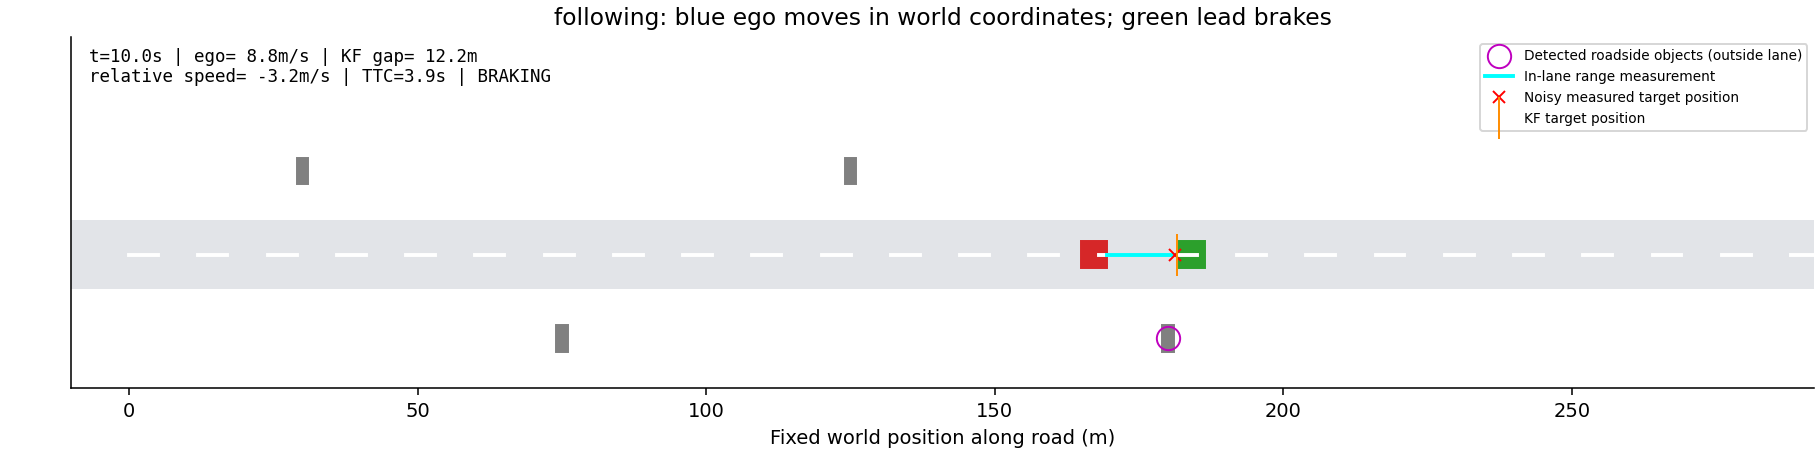
\includegraphics[width=0.988\linewidth]{assets/following_scene.png}\caption{Road simulation for the following scenario, seed 42, at 10 s. The road is fixed in world coordinates; red ego indicates braking, while gray blocks are stationary roadside objects.}\end{figure}
\begin{figure}[H]\centering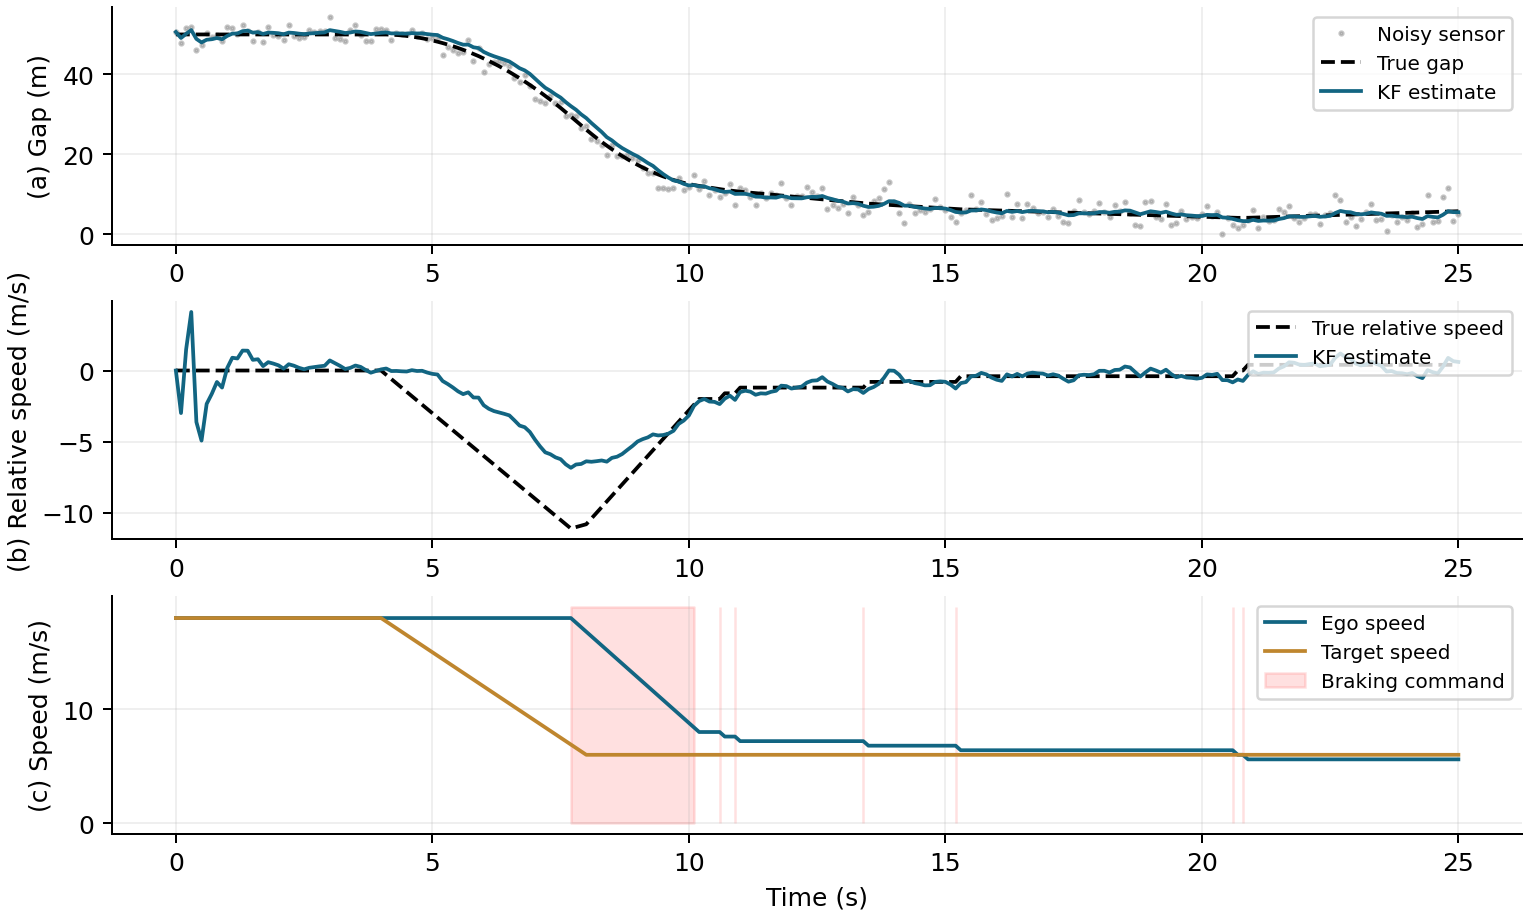
\includegraphics[width=0.975\linewidth]{assets/following_results.png}\caption{Following scenario, seed 42. (a) Distance measurements and estimates. (b) True and estimated relative speed. (c) Vehicle speeds; shaded intervals show commanded braking.}\end{figure}
Before braking, the gap is nearly constant. When the lead slows, relative speed becomes negative and the gap falls. The KF needs several observations to identify this change, so its estimate briefly lags. Ego then brakes and the closing speed decreases.\par

For this run, sensor distance RMSE is 1.877 m and KF distance RMSE is 1.057 m. The true minimum gap is 4.12 m. The controller is brake-only, so this is not a complete adaptive cruise-control system.\par

\clearpage
\needspace{4\baselineskip}\subsection{Approaching a stationary obstacle}
Ego starts at 18 m/s. A stationary in-lane obstacle is placed at 100 m. Its true speed is zero throughout the run. Roadside objects are placed at longitudinal positions 30, 75, 125 and 180 m, with lateral offsets of \ensuremath{\pm}5 m.\par

\begin{figure}[H]\centering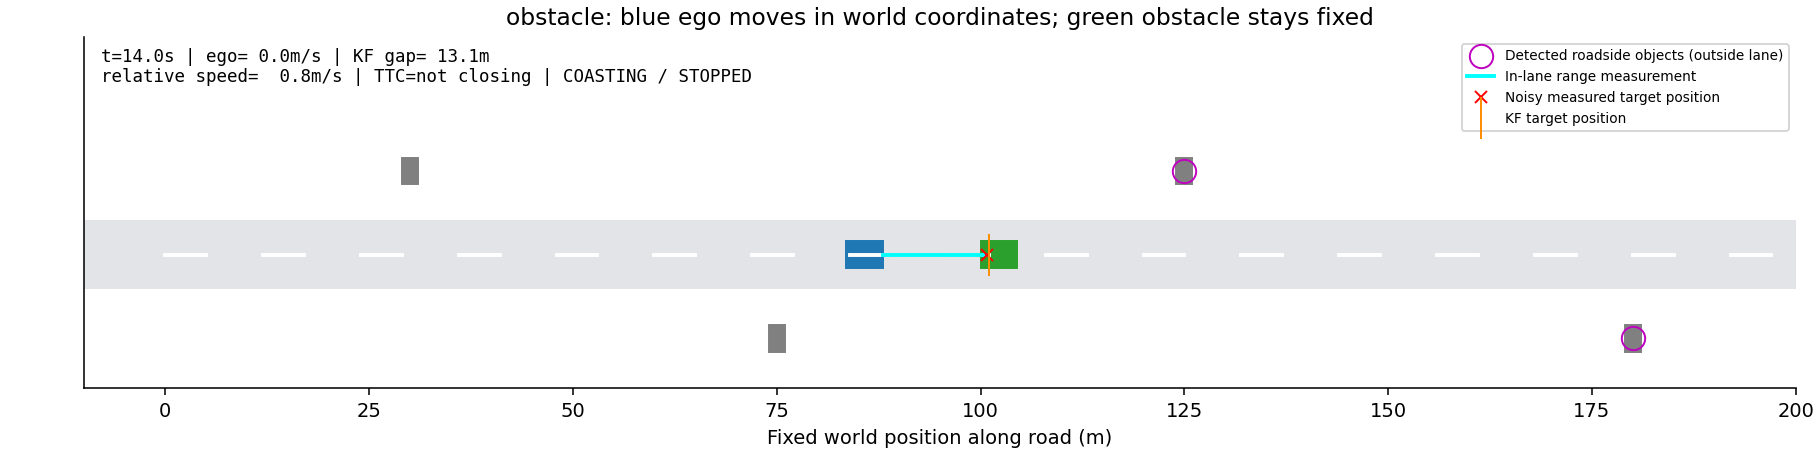
\includegraphics[width=0.988\linewidth]{assets/obstacle_scene.png}\caption{Road simulation for the obstacle scenario, seed 42, at 14 s. The road is fixed in world coordinates; red ego indicates braking, while gray blocks are stationary roadside objects.}\end{figure}
\begin{figure}[H]\centering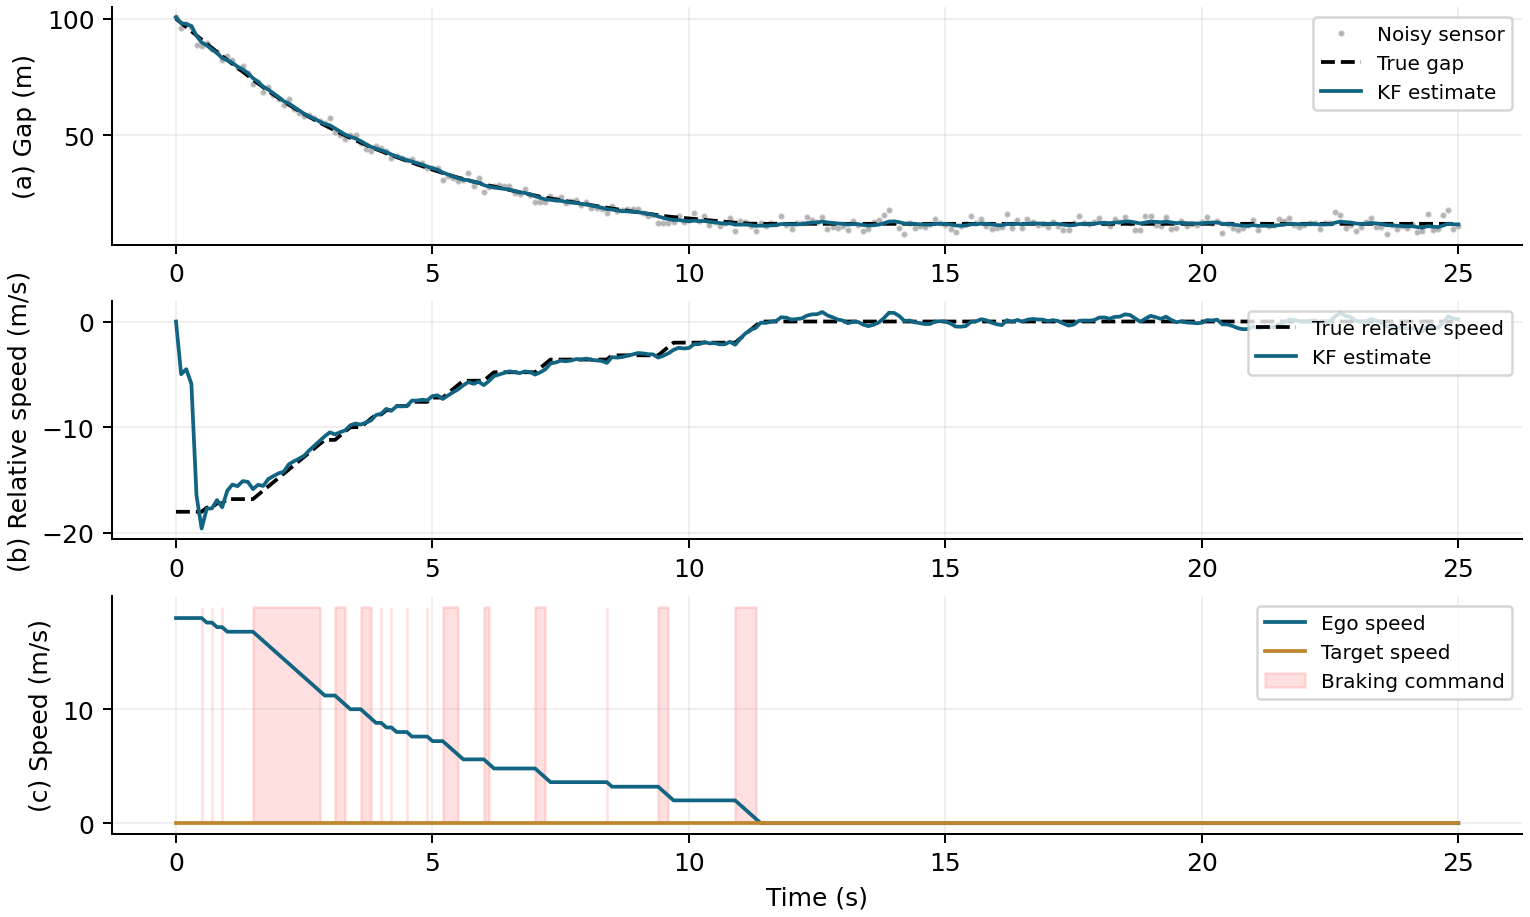
\includegraphics[width=0.975\linewidth]{assets/obstacle_results.png}\caption{Stationary-obstacle scenario, seed 42. (a) Gap to the obstacle. (b) Relative speed. (c) Ego braking to rest; the target speed remains zero.}\end{figure}
Initially, the true relative speed is -18 m/s, but the KF starts at zero because it has only one distance reading. Later readings reveal the closing speed. As braking reduces ego speed, relative speed approaches zero and the gap settles at a positive value.\par

For seed 42, ego stops with a true gap of 12.02 m. Sensor distance RMSE is 1.877 m and KF distance RMSE is 0.581 m. Small fluctuations remain even after stopping because sensor readings remain noisy.\par

\clearpage
\needspace{4\baselineskip}\subsection{Results and comparison}
Each road scenario is repeated with seeds 42 to 61. Each run has 251 samples over 25 s at 10 Hz. The sensor standard deviation is 2 m and process acceleration standard deviation is 2 m/s\textsuperscript{2}. Noise changes between seeds, and the closed-loop vehicle response may change too.\par

\begin{equation}\operatorname{RMSE}=\sqrt{\frac{1}{N}\sum_{k=1}^{N}\left(\widehat{x}_k-x_k^{\mathrm{true}}\right)^2}\end{equation}
\begin{equation}\widetilde{v}_{r,k}=\frac{z_k-z_{k-1}}{\Delta t},\qquad\sigma_{\Delta z/\Delta t}=\frac{\sqrt{2}\,\sigma_z}{\Delta t}\end{equation}
\begin{table}[H]\centering\caption{Arithmetic mean of per-run RMSE over 20 seeds. Initialisation transients are included. Raw speed uses valid successive readings only.}\small\renewcommand{\arraystretch}{1.2}\begin{tabularx}{\linewidth}{YYYYY}\toprule
\textbf{Scenario} & \textbf{Raw distance RMSE (m)} & \textbf{KF distance RMSE (m)} & \textbf{Raw speed RMSE (m/s)} & \textbf{KF speed RMSE (m/s)} \\
\midrule
Following & 2.007 & 1.206 & 28.735 & 1.733 \\
Obstacle & 2.007 & 0.697 & 28.729 & 2.041 \\
\bottomrule\end{tabularx}\end{table}
\begin{figure}[H]\centering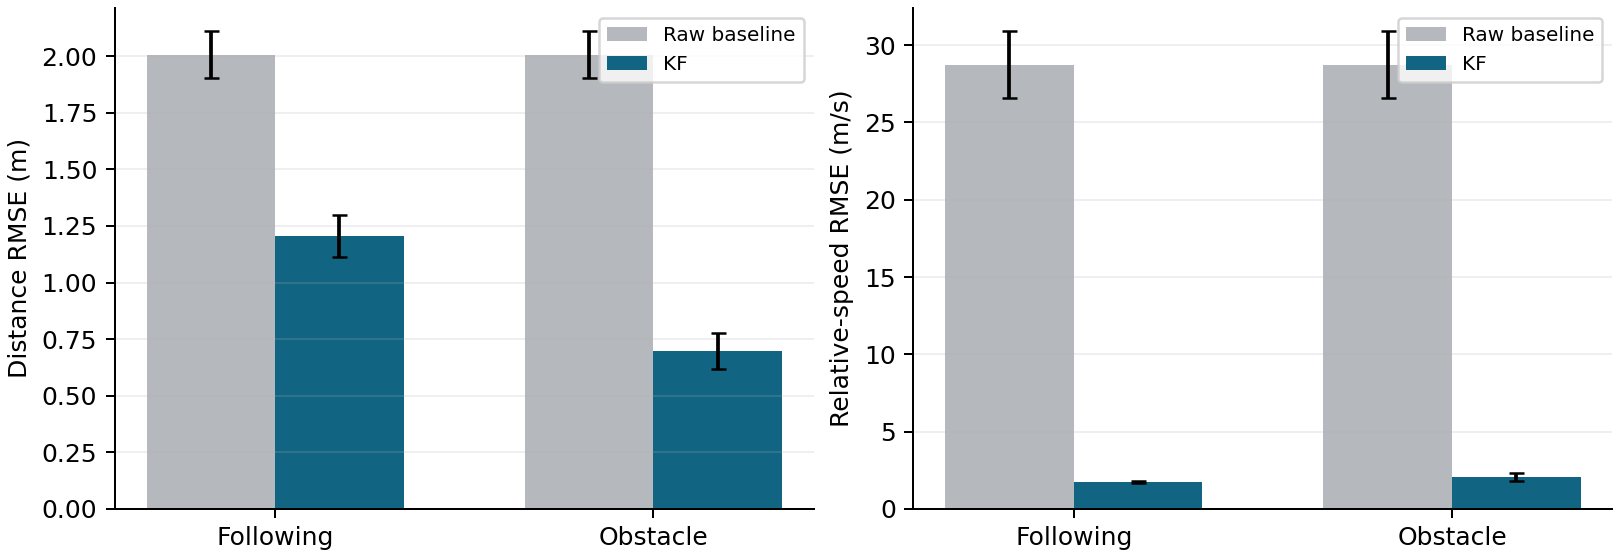
\includegraphics[width=0.988\linewidth]{assets/rmse_summary.png}\caption{Mean RMSE across 20 seeds. Error bars show one sample standard deviation of per-run RMSE, not a confidence interval.}\end{figure}
Mean range RMSE is reduced by about 40\% for following and 65\% for the stationary obstacle. Raw distance differences are much noisier than the KF speed estimate. Independent distance noise gives a difference-noise standard deviation of about sqrt(2) \ensuremath{\times} 2 / 0.1 = 28.3 m/s.\par

Both estimators are evaluated on the same driven trajectory in each trial. A separate vehicle controlled by raw readings is not simulated. The results therefore show an estimation benefit, not a measured improvement in collision rate over another controller.\par

All 40 default road runs keep a positive gap. The smallest gaps across the tested seeds are 3.72 m for following and 10.10 m for the obstacle. All 20 obstacle runs end with ego stopped. These outcomes apply to the tested conditions only.\par

\clearpage
\needspace{4\baselineskip}\subsection{Parameter tuning and sensor loss}
A supporting experiment uses the original scripted braking trajectory. Keeping that trajectory fixed helps separate filter tuning from changes caused by the feedback controller. Sensor noise stays at 2 m. The following values are means across seeds 42--61.\par

\begin{table}[H]\centering\caption{Effect of process uncertainty on the same open-loop braking experiment.}\small\renewcommand{\arraystretch}{1.2}\begin{tabularx}{\linewidth}{YYY}\toprule
\textbf{Process sigma\_\allowbreak{}a (m/s\textsuperscript{2})} & \textbf{KF distance RMSE (m)} & \textbf{KF speed RMSE (m/s)} \\
\midrule
0.5 & 2.254 & 2.148 \\
2 & 1.060 & 1.616 \\
4 & 0.882 & 1.405 \\
8 & 0.909 & 1.453 \\
\bottomrule\end{tabularx}\end{table}
A small process uncertainty strongly favours the predicted motion and can delay the response to braking. A larger value permits faster changes but can pass more noise. The values above are specific to this sampling interval and motion; there is no single setting that is best for every trajectory.\par

\begin{figure}[H]\centering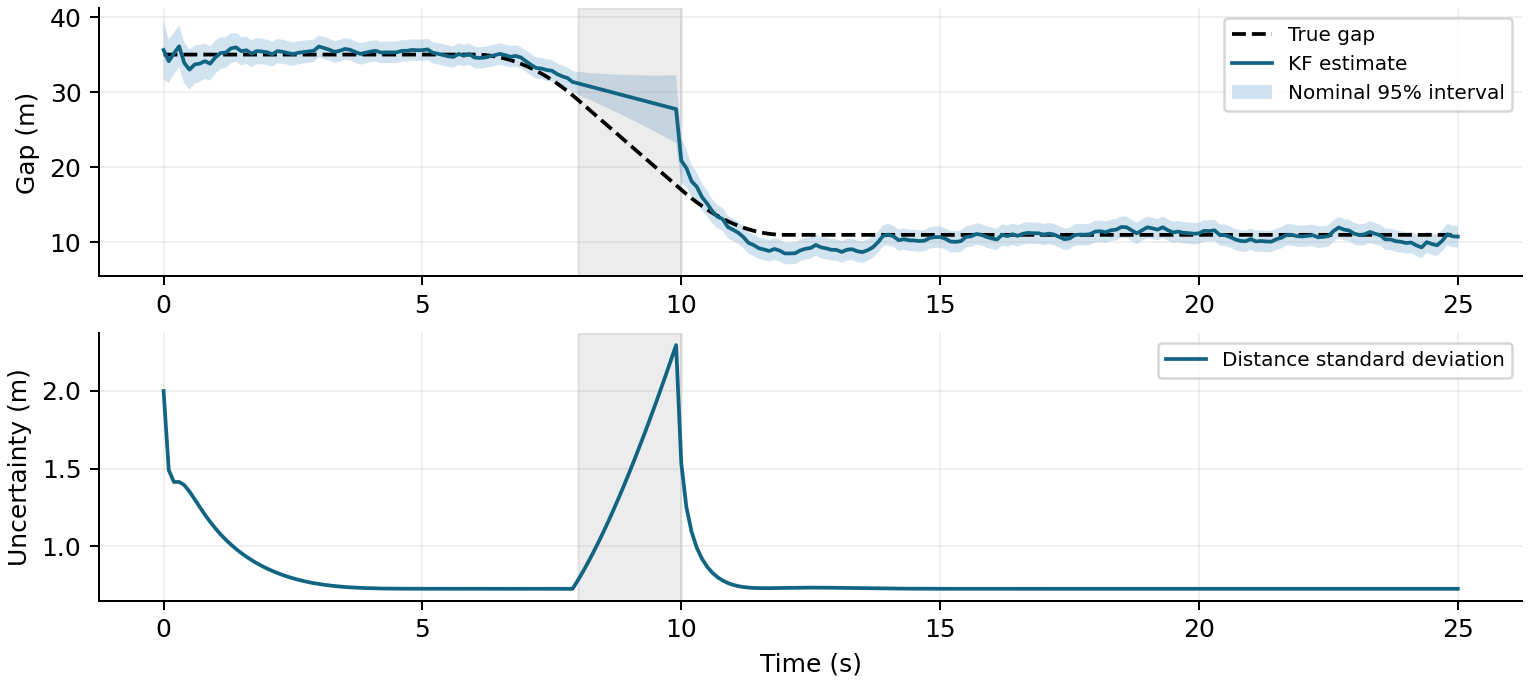
\includegraphics[width=0.975\linewidth]{assets/dropout.png}\caption{Supporting sensor-loss experiment, seed 42. The gray band marks missing measurements from 8 s to just before 10 s. Uncertainty grows during prediction-only steps.}\end{figure}
During the outage, the KF continues to predict but cannot correct its estimate. This outage overlaps braking, so the state can drift. For seed 42, full-run KF distance RMSE is 2.095 m. Raw range RMSE is 1.901 m on available samples only; the two values use different sample sets. Matched-sample errors are also exported by the program.\par

The shaded interval is a nominal Gaussian 95\% interval. It is not guaranteed to contain truth 95\% of the time when the motion model is wrong. The original 20-seed braking experiment gives about 83\% distance coverage, indicating under-estimated transient uncertainty.\par

\clearpage\section{Discussion}
\needspace{4\baselineskip}\subsection{What the KF adds}
The sensor gives distance observations. The KF combines the current observation with a prediction based on previous observations. It reduces range noise and estimates a hidden quantity, relative speed. It can also continue predicting briefly when observations are missing. These are useful inputs to a safety decision.\par

The filter does not identify an obstacle by itself. Detection, state estimation and control are separate tasks. Here the simulator supplies the target identity and lane label. One KF follows the in-lane target. Roadside detections are logged but are not fused into that target track.\par

\needspace{4\baselineskip}\subsection{Limits of this study}
Motion is one-dimensional. There are no curves, steering decisions, intersections or maps. Sensor noise is Gaussian with known variance. There are no clutter returns, incorrect lane labels or changing object identities. The controller assumes ideal braking with no actuator delay, tyre model or road-friction limit.\par

The KF assumes near-constant relative velocity between updates, apart from known ego acceleration. Strong target braking causes lag. At start-up, speed is uncertain. During long outages, prediction can become inaccurate. TTC assumes unchanged relative speed and is sensitive near zero closing speed.\par

\needspace{4\baselineskip}\subsection{Verification}
Seven automated tests check constant-speed convergence, prediction without measurements, repeatability and valid covariance, TTC signs, invalid parameters, known acceleration input, and road outcomes across 20 seeds per scenario. All pass. Frames from both road animations and GIF exports have also been checked.\par

\clearpage\section{Conclusion}
A two-state linear KF is suitable for this simplified longitudinal tracking problem. The measured results show lower distance error and much lower speed noise than simple raw baselines. The road demonstrations explain how those estimates can support braking. The tuning and dropout experiments show why assumptions and uncertainty still matter.\par

Further work could use real range recordings, test incorrect noise settings, add acceleration to the state, and compare controllers under the same disturbances. Multiple objects would require separate tracks and measurement association. Steering avoidance would also require lateral motion and path planning.\par

\end{document}